% Chapter 3

\chapter{Project 2b: Radix sort} % Main chapter title

\label{Chapter3} % Change X to a consecutive number; for referencing this chapter elsewhere, use \ref{ChapterX}

\lhead{Chapter 3. \emph{Radix sort}} % Change X to a consecutive number; this is for the header on each page - perhaps a shortened title

%----------------------------------------------------------------------------------------


\section{Introduction}



\section{Implementations}




\subsection{Counting sort (CS)}
We start by finding the greatest value in the list gKey.
gKey = Max(Array)+1
We use gKey to create a new array C and for every entry in C we set the value to 0.
in line 4-5 we go through the input array and use the c array as a histogram so for all the elements i array we go to the equvalent index in C and increase it by 1.

\lstinputlisting[language=C++, firstline=32, lastline=46, numbers=left]{./Figures/CountingSort.cpp}

\subsection{Quick sort (QS)}
\lstinputlisting[language=C++, firstline=13, lastline=16, numbers=left]{./Figures/QuickSort.cpp}
\lstinputlisting[language=C++, firstline=20, lastline=21, numbers=left]{./Figures/QuickSort.cpp}


\subsection{Most significant digit (MSD)}

The MSD radix sort is implemented as follows:
\begin{verbatim}
  // Pass 0
  queue<int> buckets[N_BUCKETS];
  for (int i = 0; i < arrSize; i++) {
    // Add to bucket
    buckets[ sortedArray[i] >> (K-D) ].push(sortedArray[i]);
  }
  // Pass 1 (and the rest, recursively)
  for (int b = 0; b < N_BUCKETS; b++) {
    msdRecursive(buckets[b], 1);
  }
  return sortedArray;
\end{verbatim}


It makes use of the following recursive method:
\begin{verbatim}
void msdRecursive(queue<int> bucket, int pass) {
  if (bucket.empty()) return;
  
  // Base case (this bucket is already fully sorted).
  if (pass == N_PASSES) {
    while(!bucket.empty()) {
      sortedArray[sortArrIdx] = bucket.front();
      bucket.pop();
      sortArrIdx++;
    }
    return;
  }
  // Sort this bucket into some new buckets.
  queue<int> buckets[N_BUCKETS];
  while(!bucket.empty()) {
    const int key = bucket.front();
    bucket.pop();
    // Add to bucket
    buckets[ (key >> (K - (pass+1)*D)) & MASK_D ].push(key);
  }
    // Example (K=8, D=2, pass=1, so we have already sorted by AB, and now we look at CD):
    // (ABCDEFGH >> (8 - (1+1)*2)) & 00000011
    // (ABCDEFGH >> 4) & 00000011
    //  0000ABCD & 00000011
    //  000000CD

  // Now, sort all buckets recursively.
  for (int b = 0; b < N_BUCKETS; b++) {
    msdRecursive(buckets[b], pass+1);
  }
}
\end{verbatim}



\subsection{Least significant digit (LSD)}


\subsection{MSD - using arrays (MSD\_arr)}


\subsection{LSD - using arrays (LSD\_arr)}
This version has not been implemented, but it could be done by making similar modifications to LSD as above.


\subsection{Multicore radix sort (MCR) \citep{radixSort}}



\section{Results and discussion}


\begin{figure}[htbp]
	\centering
		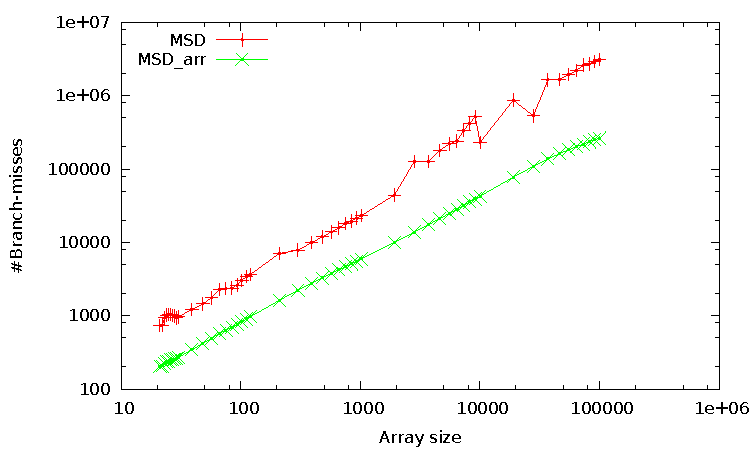
\includegraphics[width=\textwidth]{./Figures/Project2b/Branch_misses.pdf}
		\rule{35em}{0.5pt}
	\caption[Branch misses]{
	Bla bla bla.
	}
	\label{fig:Branch_misses}
\end{figure}


\begin{figure}[htbp]
	\centering
		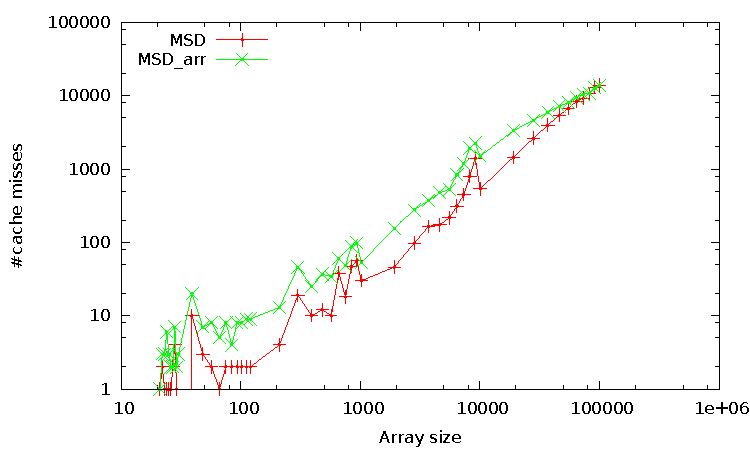
\includegraphics[width=\textwidth]{./Figures/Project2b/Cache_misses.pdf}
		\rule{35em}{0.5pt}
	\caption[Cache misses]{
	Bla bla bla.
	}
	\label{fig:Cache_misses}
\end{figure}



\begin{figure}[htbp]
	\centering
		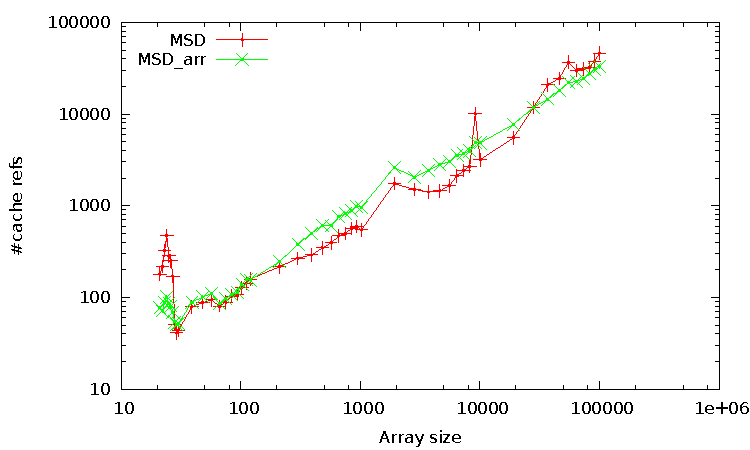
\includegraphics[width=\textwidth]{./Figures/Project2b/Cache_refs.pdf}
		\rule{35em}{0.5pt}
	\caption[Cache refs]{
	Bla bla bla.
	}
	\label{fig:Cache_refs}
\end{figure}



\begin{figure}[htbp]
	\centering
		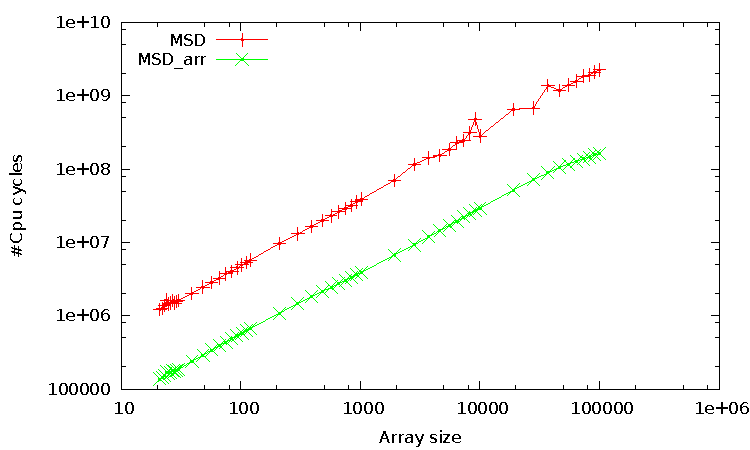
\includegraphics[width=\textwidth]{./Figures/Project2b/Cpu_cycles.pdf}
		\rule{35em}{0.5pt}
	\caption[CPU cycles]{
	Bla bla bla.
	}
	\label{fig:Cpu_cycles}
\end{figure}


\begin{figure}[htbp]
	\centering
		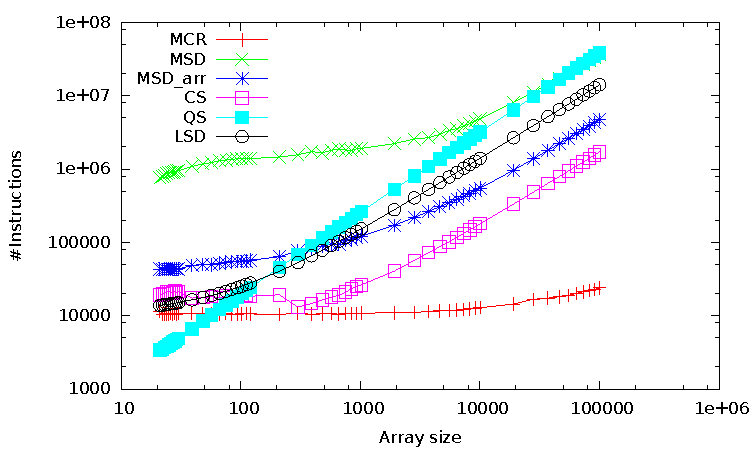
\includegraphics[width=\textwidth]{./Figures/Project2b/Instructions.pdf}
		\rule{35em}{0.5pt}
	\caption[Instructions]{
	Bla bla bla.
	}
	\label{fig:Instructions}
\end{figure}

\begin{figure}[htbp]
	\centering
		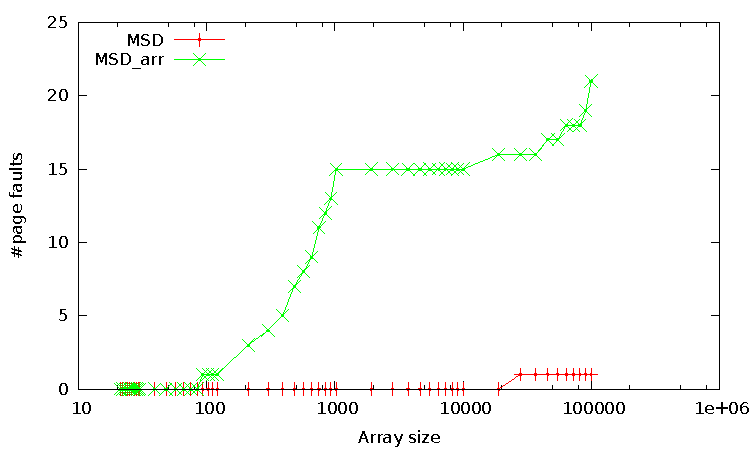
\includegraphics[width=\textwidth]{./Figures/Project2b/Page_faults.pdf}
		\rule{35em}{0.5pt}
	\caption[Page faults]{
	Bla bla bla.
	}
	\label{fig:Page_faults}
\end{figure}


